\documentclass{beamer}
\usepackage[T2A]{fontenc}
\usepackage[utf8]{inputenc}
\usepackage[english, russian]{babel}
\usepackage{graphicx}
\graphicspath{{images/}}

\usetheme{Madrid}
\usecolortheme{beaver}

\title{О математическом моделировании процесса погружения сваи с дополнительными параметрами}
\date{02.07.2025}
\author{Бабошин Сергей Дмитриевич}

\setbeamertemplate{frametitle}[default][center]
\setbeamertemplate{navigation symbols}{}
\setbeamertemplate{footline}[page number]
\setbeamertemplate{caption}[numbered]

\begin{document}

    \frame{\titlepage}

    \begin{frame}
        \frametitle{Постановка задачи}
        В данной работе ставятся и решаются следующие задачи:
        \begin{enumerate}
            \item Описать математическую модель процесса работы импульсного погружателя с дефектами;
            \item Оценить суммарное влияние, вносимое деталями с дефектами и естесвенным износом на процесс погружения;
            \item Оценить влияние на процесс погружения, вносимое каждой парой дебалансов в отдельности.
        \end{enumerate}
    \end{frame}

    \begin{frame}
        \frametitle{Импульсный погружатель}
        \begin{figure}
            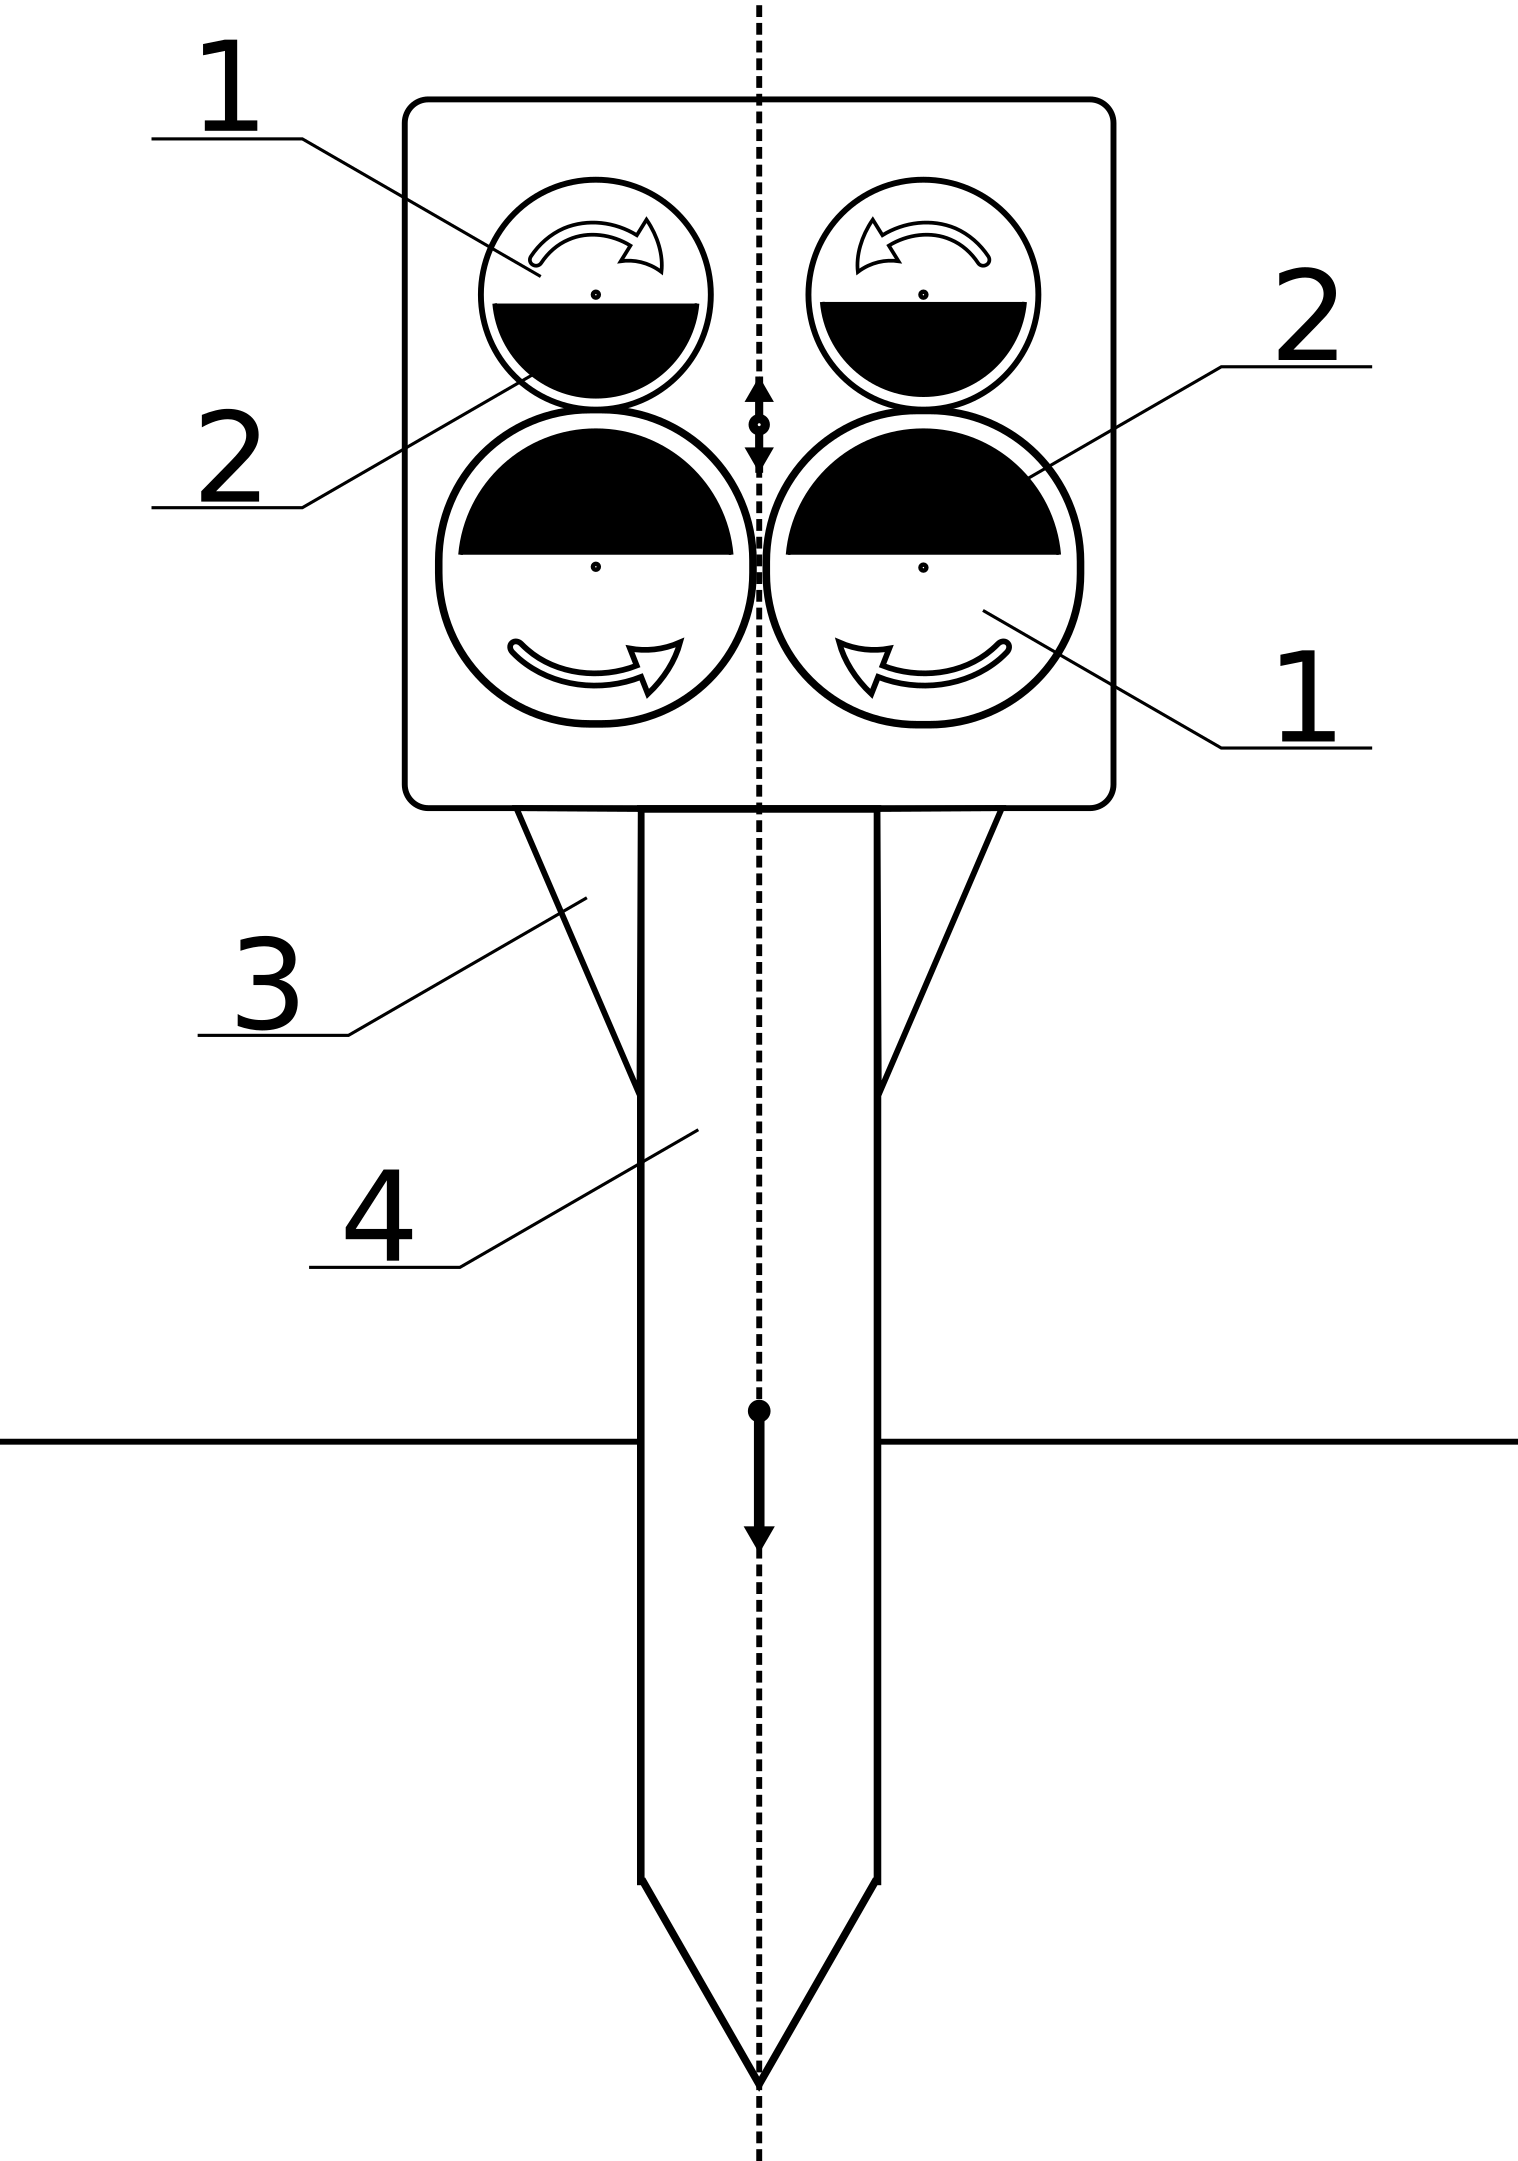
\includegraphics[width=0.4\linewidth]{pogruzhatel-2}
            \caption{Модель импульсного погружателя.}
        \end{figure}
    \end{frame}

    \begin{frame}
        Сила, генерируемая импульсным погружателем:
        \begin{equation}
            f(t,\lambda)=\sum_{k=1}^n \lambda_k\cos(kt),\ t\in [-\pi,\pi],\ \lambda =(\lambda_1, \ldots,\lambda_n).
        \end{equation}
        \begin{figure}
            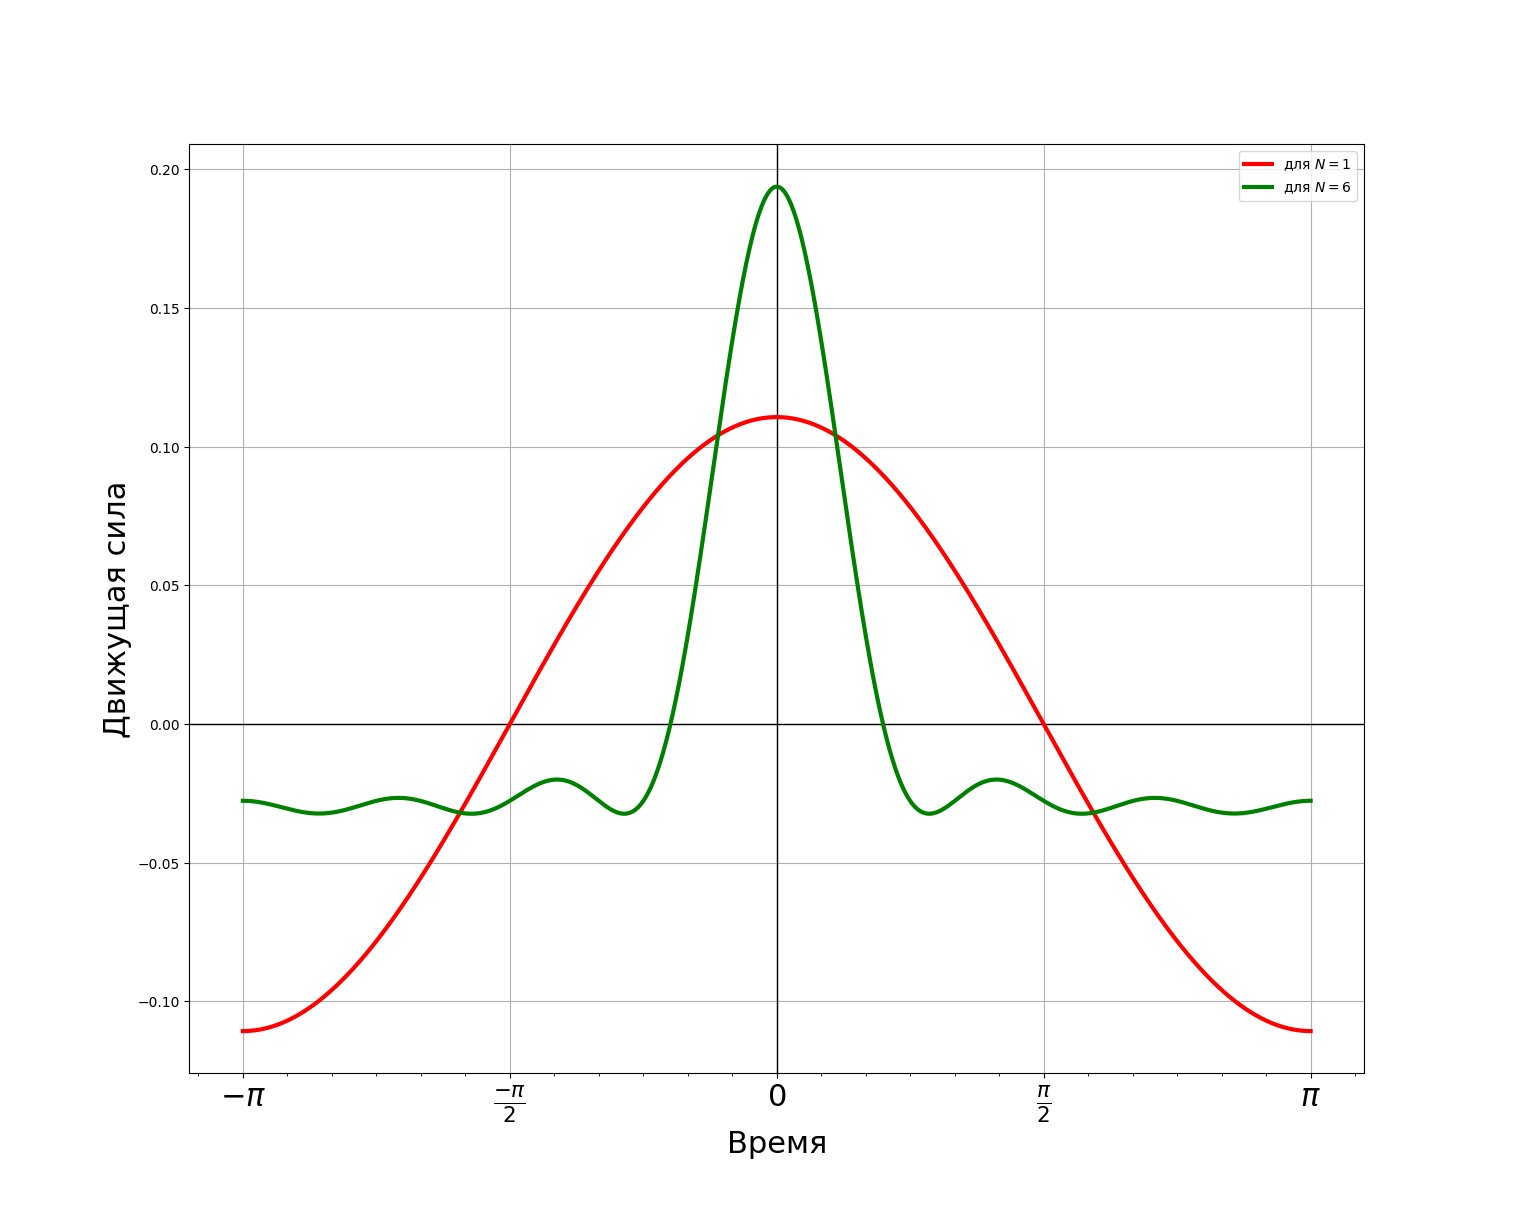
\includegraphics[width=0.75\linewidth]{impulse_1vs6}
        \end{figure}
    \end{frame}

    \begin{frame}
        Уравнение гармонического колебания пары дебалансов будет иметь вид:

        \begin{equation}
            \begin{aligned}
                x(t) = 2 m \omega^2 l \cos (\omega t)
            \end{aligned}
        \end{equation}
        \noindent где $m$ - масса дебаланса, $l$ - расстояние от центра масс до оси вращения дебаланса, $\omega$ - угловая скорость.

        \noindent Для всех пар дебалансов сумма гармонических колебаний будет иметь вид:

        \begin{equation}
            \label{eq:F}
            F = \sum\limits_{k = 1}^n 2 m_k \cdot (k \omega)^2 \cdot l(r_k) \cdot \cos (k \omega t)
        \end{equation}
        \noindent где $n$ --- количество пар дебалансов, $k$ --- порядковый номер пары дебалансов.
    \end{frame}

    \begin{frame}
        Абсолютное отношение максимального значения функции к минимальному значению называется коэффициентом асимметрии $K_n$:
        \begin{equation}
            \label{eq:asymm-coef}
            K_n = \left| \frac{ \max\limits_{-\pi<t<\pi} F(t)}{\min\limits_{-\pi<t<\pi} F(t)}\right|,
        \end{equation}

        Модель оптимального импульсного погружателя:
        \begin{equation}
            \label{eq:impulse_mf}
            f_n(t, \lambda) = \sum\limits_{k = 1}^n (n-k+1) \cos(k \omega t),\ t \in [-\pi, \pi],\ \lambda =(\lambda_1, \ldots,\lambda_n)
        \end{equation}

        Функция (\ref{eq:impulse_mf}) называется импульсом Максвелла–Фейера.
    \end{frame}

    \begin{frame}
        \begin{figure}[ht]
            \centering
            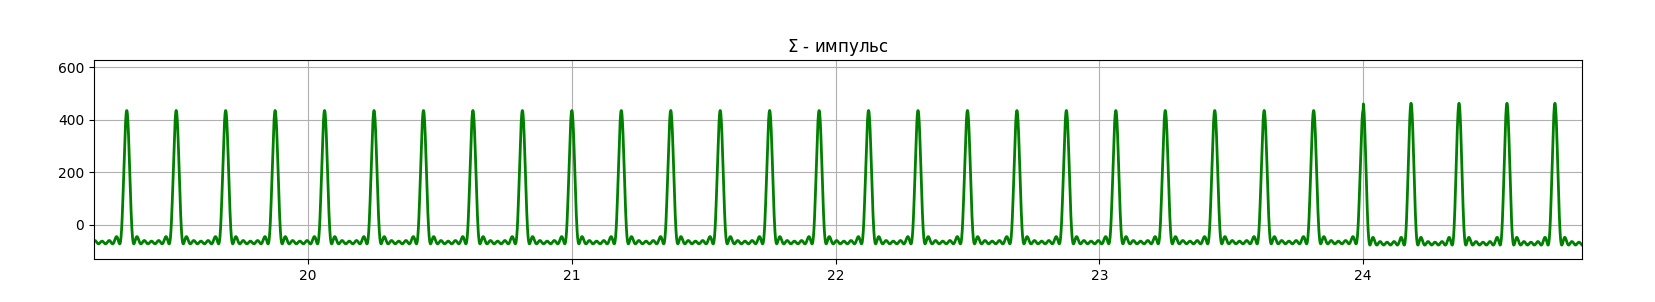
\includegraphics[width=1\linewidth]{graph-impulse}
            \caption{Оптимальный импульс, создаваемый импульсным погружателем.}
            \label{fig:graph-impulse}
        \end{figure}
    \end{frame}

    \begin{frame}
        \frametitle{Моделирование процесса погружения}
        Процесс вибрационного погружения можно описать с помощью следующего равенства:
        \begin{equation}
            \label{eq:R}
            R = F_\text{вибр. возд.} + F_\text{тяж.} - F_\text{бс} - F_\text{лс},
        \end{equation}
        Расписав \ref{eq:R} более подробно получаем следующее ДУ:
        \begin{equation}
            \label{eq:main}
            m\ddot{x} = F_\text{вибр. возд.} + mg - P x(t) f_i(\psi) - S_\text{пс} h_i(x(t), \xi)
        \end{equation}
        с начальными условиями:
        \begin{equation*}
            x(0) = 0, \dot{x}(0) = 0.
        \end{equation*}
        Где $m$ -- масса всей установки, $x(t)$ -- глубина погружения сваи, $t$ -- время погружения сваи.
    \end{frame}

    \begin{frame}
        \frametitle{Численное решение}
        Рассмотрим разностную аппроксимацию дифференциального оператора $L_{xx} = \ddot{x}$ на равномерной сетке с шагом $h$:
        \begin{equation}
            \label{eq:lxx}
            L_{xx} = \ddot{x} = \frac{x(t + h) - 2x(t) + x(t - h)}{h^2}
        \end{equation}
        Заменив $\ddot{x}$ в уравнении \ref{eq:main} разностной аппроксимацией \ref{eq:lxx}, получаем:
        \begin{equation*}
                x_{i+1} = 2x_i - x_{i-1} + \frac{h^2}{m}(F_\text{вибр. возд.} + mg + S_\text{пс} h_i(x(t), \xi) + P x(t) f_i(\psi)),
        \end{equation*}
        где $x_i = x(t_i)$ и 
        \begin{equation*}
            x_0 = 0, x_1 = 0
        \end{equation*}
        Данное рекурентное равенство лежит в основе расчёта глубины погружения.
    \end{frame}

    \begin{frame}
        \frametitle{Программа для расчёта процесса погружения}
        \begin{figure}
            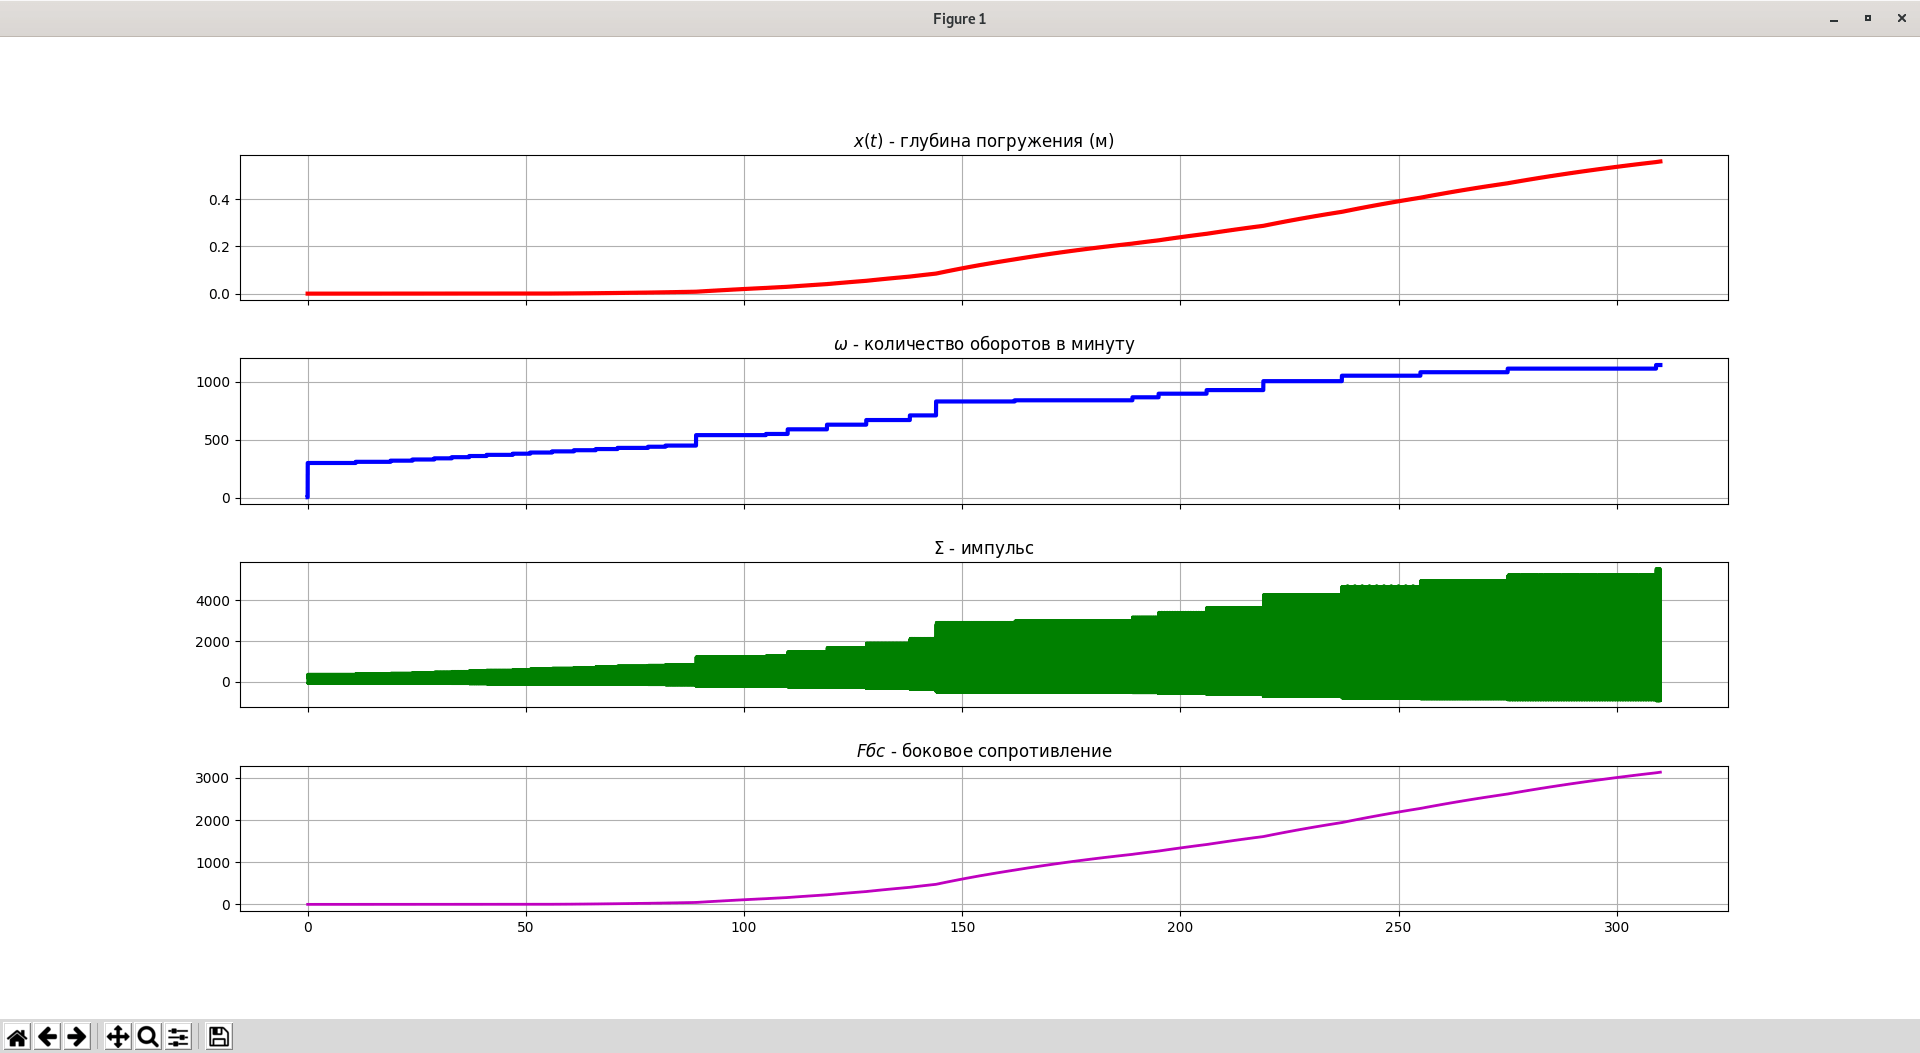
\includegraphics[width=1\linewidth]{screenshot}
            \caption{Скриншот окна программы.}
        \end{figure}
    \end{frame}

    \begin{frame}
        \frametitle{Допуски на изготовление и естесвенный износ}

        Допуски на производстве и естесвенный износ деталей погружателя приводят к следующей модели:
        \begin{equation}
            \widetilde{\omega} = \omega (1 + \delta(t)),
        \end{equation}
        где $\delta(t)$ - погрешность угловой скорости вращения вала дебаланса в момент времени $t$, вызванная дефектами узлов погружателя.

        Т.о. выражение (\ref{eq:F}) примет вид:

        \begin{equation}
            \label{eq:F_noise}
            \begin{gathered}
                F = \sum\limits_{k = 1}^n 2 m_k \cdot (k \omega (1 + \delta(t)))^2 \cdot l(r_k) \cdot \cos (k \omega (1 + \delta(t)) t)
            \end{gathered}
        \end{equation}
    \end{frame}

    \begin{frame}
        \begin{figure}[ht]
            \centering
            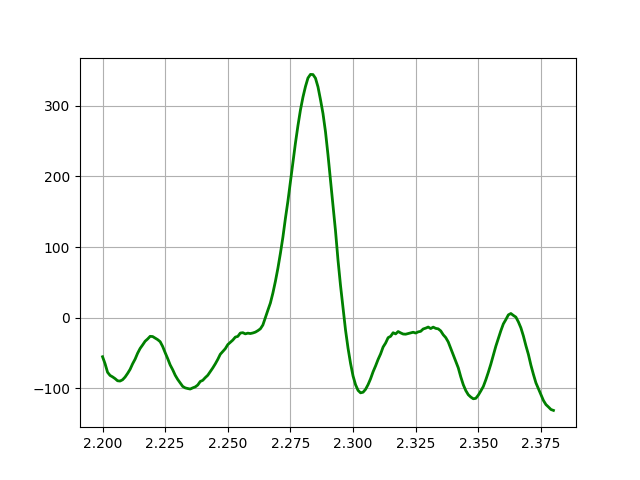
\includegraphics[width=0.33\linewidth]{noise_001}
            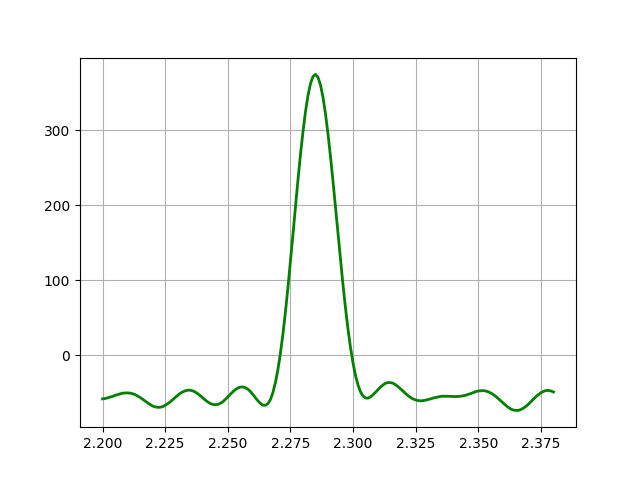
\includegraphics[width=0.33\linewidth]{noise_0001}

            a. $\sigma = 10^{-2}$ \hspace{2cm} b. $\sigma = 10^{-3}$

            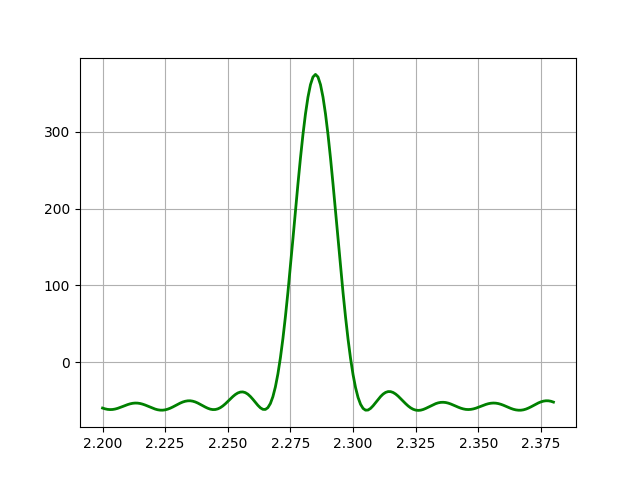
\includegraphics[width=0.33\linewidth]{noise_00001}
            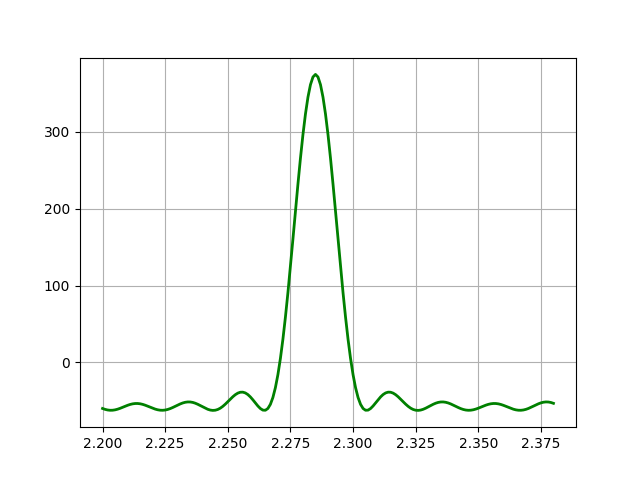
\includegraphics[width=0.33\linewidth]{noise_0}

            c. $\sigma = 10^{-4}$ \hspace{2cm} d. $\sigma = 0$
            \caption{График импульса вынуждающей силы.
            $a$ -- в поле шума со стандартным отклонением $\sigma = 10^{-2}$;
            $b$ -- в поле шума со стандартным отклонением $\sigma = 10^{-3}$;
            $c$ -- в поле шума со стандартным отклонением $\sigma = 10^{-4}$;
            $d$ -- идеальный случай, без шума.}
            \label{fig:impulse-noise}
        \end{figure}
    \end{frame}

    \begin{frame}
        \begin{figure}[ht]
            \centering
            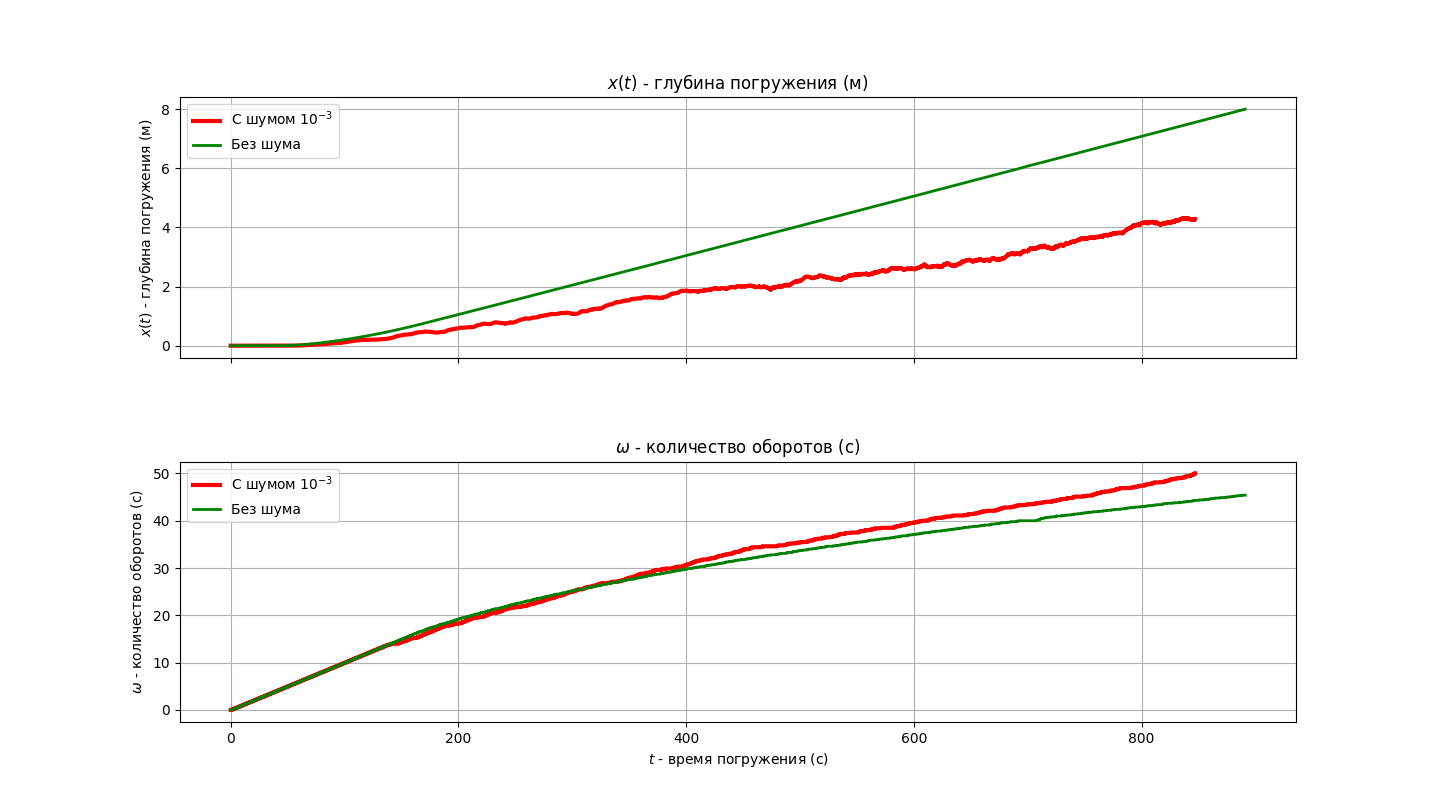
\includegraphics[width=1\linewidth]{dive_with_noise}
            \caption{Графики угловых скоростей и глубины погружения сваи в грунт.
            Зеленый -- идеальный случай; красный -- поле шума со стандартным отклонением $\sigma = 10^{-3}$}
            \label{fig:dive_with_noise}
        \end{figure}
    \end{frame}

    \begin{frame}
        \frametitle{Влияние каждой пары дебалансов с дефектами}
        Вынуждающая сила импульсного погружателя, при наличии отклонения в угловой скорости $m$-го дебаланса:
        \begin{equation}
            \label{eq:F_noise_one_deb}
            \widetilde{F} = \sum\limits_{k = 1}^n (n - k + 1) \cdot \cos (k \omega (1 + \delta_k) t),
        \end{equation}
        где
        \begin{equation}
            \begin{aligned}
                \delta_k =
                \begin{cases}
                    0, \quad k \neq m \\
                    \varepsilon, \quad k = m,
                \end{cases}
            \end{aligned}
        \end{equation}
    \end{frame}

    \begin{frame}
        \begin{figure}[ht]
            \centering
            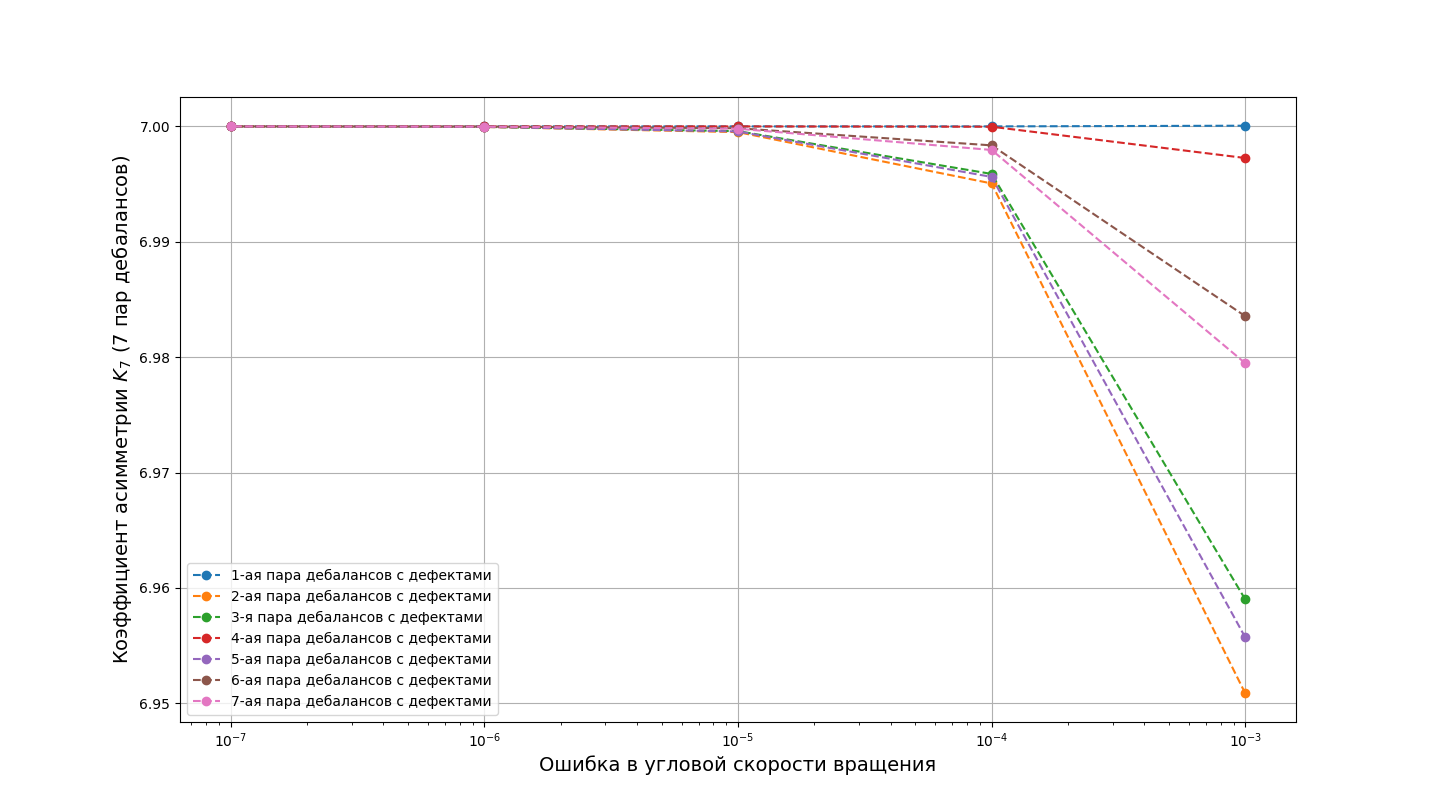
\includegraphics[width=1\linewidth]{pairs_with_defects_7}
            \caption{График изменения коэффициента ассиметрии для каждой пары дебалансов и погрешностей изготовления.
            Количество пар дебалансов -- 7.}
            \label{fig:pairs_with_defects_7}
        \end{figure}
    \end{frame}

    \begin{frame}
        \begin{figure}[ht]
            \centering
            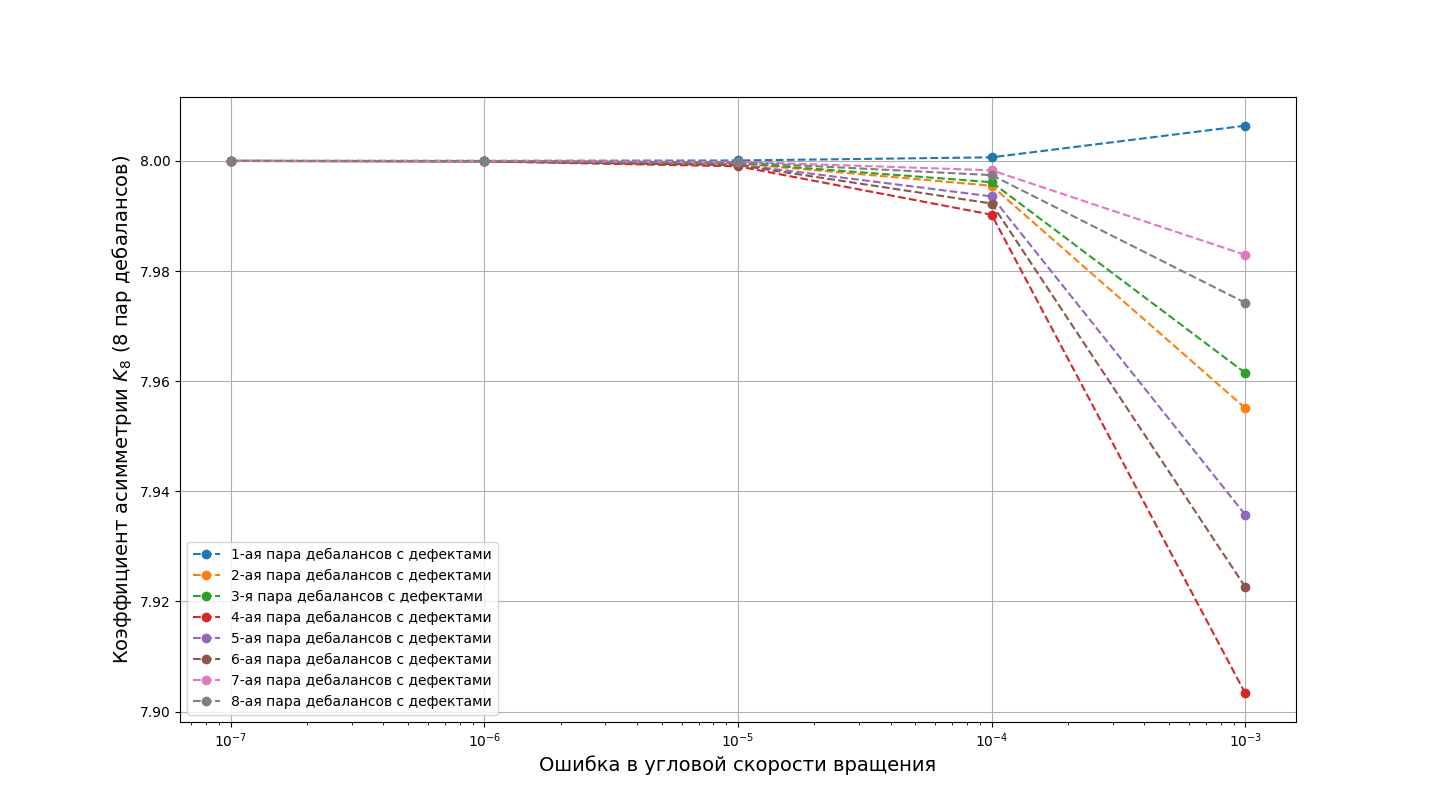
\includegraphics[width=1\linewidth]{pairs_with_defects_8}
            \caption{График изменения коэффициента ассиметрии для каждой пары дебалансов и погрешностей изготовления.
            Количество пар дебалансов -- 8.}
            \label{fig:pairs_with_defects_8}
        \end{figure}
    \end{frame}

    \begin{frame}
        \begin{alertblock}{}
            \centerline{\color{darkred}Спасибо за внимание!}
        \end{alertblock}
    \end{frame}

\end{document}